\label{sect:architecture}
\section{Design and Implementation}
%As previously mentioned, there has been great interest in scientific named entity recognition (NER), especially in the fields of biomedicine.  
%It is even more challenging for new fields to leverage existing machine learning methods without access to large amounts of labeled training data.
%We develop a framework to efficiently retrieve and classify scientific named
%entities. 
PolyNER uses word representations and minimal domain knowledge (a few
seed entities) to produce a small set of candidates for expert labeling;
labeled candidates are then used to train named entity word vector classifiers.
We implement an active learning loop in order to incrementally improve the performance of the classifiers.
\kyle{Come back to this. Not sure if it belongs here or in eval yet.}
In order to explore whether natural language processing, and specifically the use of word vector coordinates as features can accelerate the learning process,
we use three sampling strategies and two different candidate pools for maximum entropy uncertainty sampling, which we describe in this section.
The general architecture of polyNER is illustrated in Figure~\ref{fig:architecture}.
We also describe the labeling process, training and testing set up for our word vector classifiers in the active learning loop. 

\begin{figure*}[!t]
{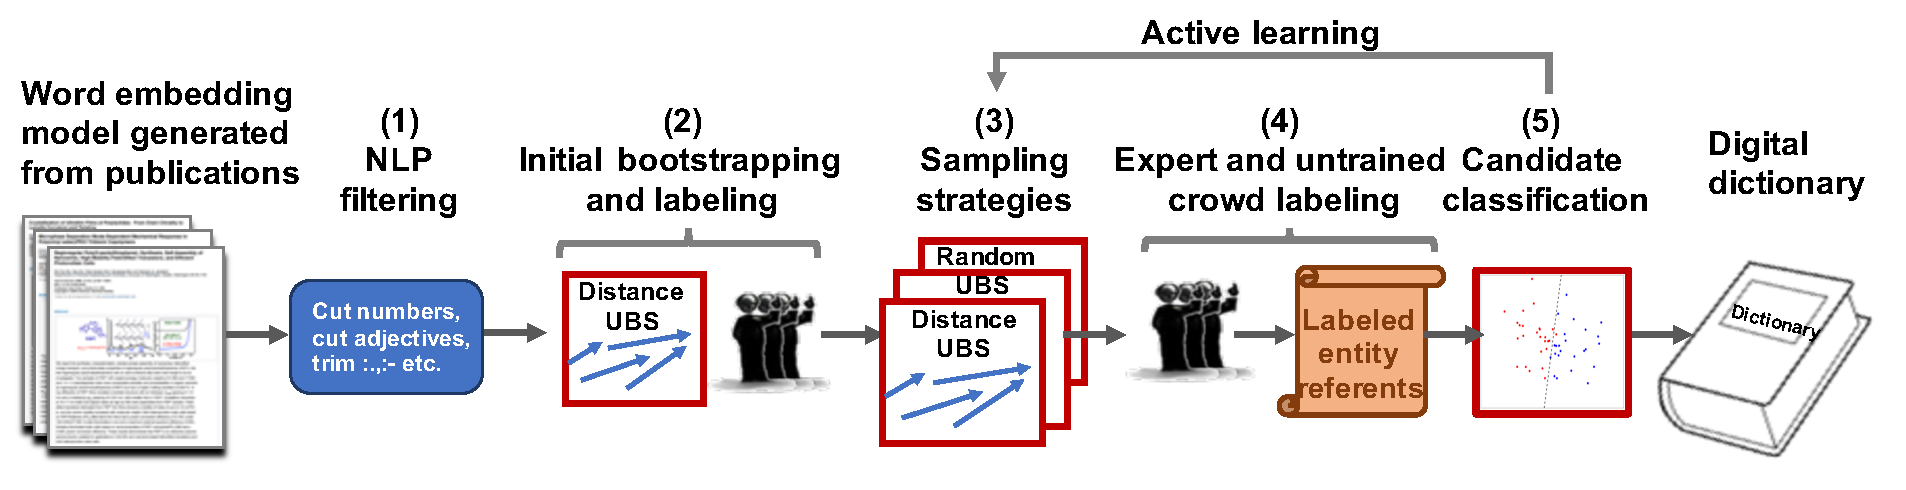
\includegraphics[width=\textwidth]{figures/architecture.pdf}}
\caption{\label{fig:architecture} PolyNER system showing NLP-filtering in (1), candidate sampling strategies in (2), and actie learning loop between expert labeling (3) and classification of scientific named entities (4). 
}
\end{figure*}

\subsection{Preprocessing}
First, we define an
NLP filtering preprocessing step that is used to filter out
words in scientific publications that are unlikely to be polymer referents. 1) We remove numbers. 2)
Hypothesizing that names of scientific entities will not, in general, be English
vocabulary words, we remove words found in the SpaCy dictionaries
of commonly used English words~\cite{choi2015depends}. (We manually remove common polymer
names, such as polystyrene and polyethylene, from the dictionaries.) 3) We use
SpaCy's part-of-speech tagging functionality to remove non-nouns. 4)We remove
unwanted characters (e.g. `:', `.', `,', `:', `-') from the beginning and the end of each
candidate, allowing us to recognize, for example, polyethylene; (which fails the
exact string comparison test against ``polyethylene''). 5) We remove plurals (e.g.,
polyamides, polynorbornenes), as they can represent polymer family names.
We refer to these pre-processed words (output of step 1 in Figure~\ref{fig:architecture}) as NLP-filtered candidates.



\subsection{Labeling Strategies}
%\kyle{We should think about how to structure this. It seems like we want to outline
%the normal process and then perhaps introduce some baselines for comparison in the next section.}\roselyne{I'll leave this here and make a note to talk but I think we don't have much to gain comparing these since we started them all with th distance candidates. Hope it still makes sense this way.}

We implement three sampling strategies, which we refer to as \textit{Random}, \textit{AL1} and \textit{AL2}, 
to determine which candidates to label.
Based on preliminary experiment, we set the size of batches of strings to be labeled to 200 or about an hour of expert time.\\

\subsubsection{Random Strategy}
In the first strategy we randomly select 200 out of the pool of unlabeled NLP-filtered candidates.
%\kyle{not known what an unlabeled NLP-filtered candidate is}. 
Note that the imbalance between polymers and other \textit{tokens} (words or space separated strings) that do not exist in in this set is still significant (less than 5\% in our test set).\\

\subsubsection{Active Learning using NLP-Filtered Candidates (AL1)}
In the second strategy we use maximum entropy sampling method using the same pool of NLP-filtered candidates.
As previously mentioned, maximum entropy selection falls under the category of uncertainty sampling, which identifies data points where a classifier predicts outcome at the decision boundary between two or more classes. 
For example, in our case, when predicting whether a word vector represents a polymer, or not, the classifier assigns equal probability to either case.
In the binary case, probabilities range from $0$ to $0.5$ or 50\%. Therefore, we predict outcome for all our NLP-filtered candidates and obtains a probability $p$ for each data point. We compute a list of $0.5-p$ values for all unlabeled data and sort the list in ascending order.
Points with scores closest to $0$ are most uncertain, we select the first 200 entries from this ordered list to be labeled by experts.\\


\subsubsection{Active Learning using NLP-Filtered Distance Candidates (AL2)}
Finally, the third pool is composed of NLP-filtered candidates deemed to be most similar to seed entities using vector similarity measures.
The intuition behind generating this pool of candidates is to increase the likelihood that a candidate is a target referent (name, acronym, synonym, etc.) by comparing its vector to that of a known entity.
Our goal is to determine whether polymers are used in a consistent context that can be used to detect and classify their corresponding context-aware vectors.
For example, the polymer name ``polystyrene'' in a sentence ``The
melting point of polystyrene is ...'' suggests that X may also be a polymer in the
sentence ``The melting point of X is ...''.
A word embedding method maps each word
in a sentence or document to a vector in an n-dimensional real vector space
based on the linguistic context in which the word appears. (This mapping may
be based, for example, on co-occurrence frequencies of words.) 
We can then
determine the similarity between two words by computing the distance between
their corresponding vectors in the feature space.
We use Word2Vec, a recent, light-weight and easy-to-use implementation of context-based vector representations~\cite{mikolov2013efficient,mikolov2013distributed}.
Specifically we use the Gensim continuous bag-of-words
(CBOW) implementation of the Word2Vec
algorithm~\cite{rehurek2010software} to generate vectors.
We can then determine, for each NLP-filtered word, the extent to which it occurs
in a similar context to the representative polymers, by computing the similarities
between the word's vector and those for our seed entities. 
When dealing with multiple seed entities, we use the highest similarity score for ranking candidates.

\begin{figure*}[!t]
\centering
\scalebox{0.6}{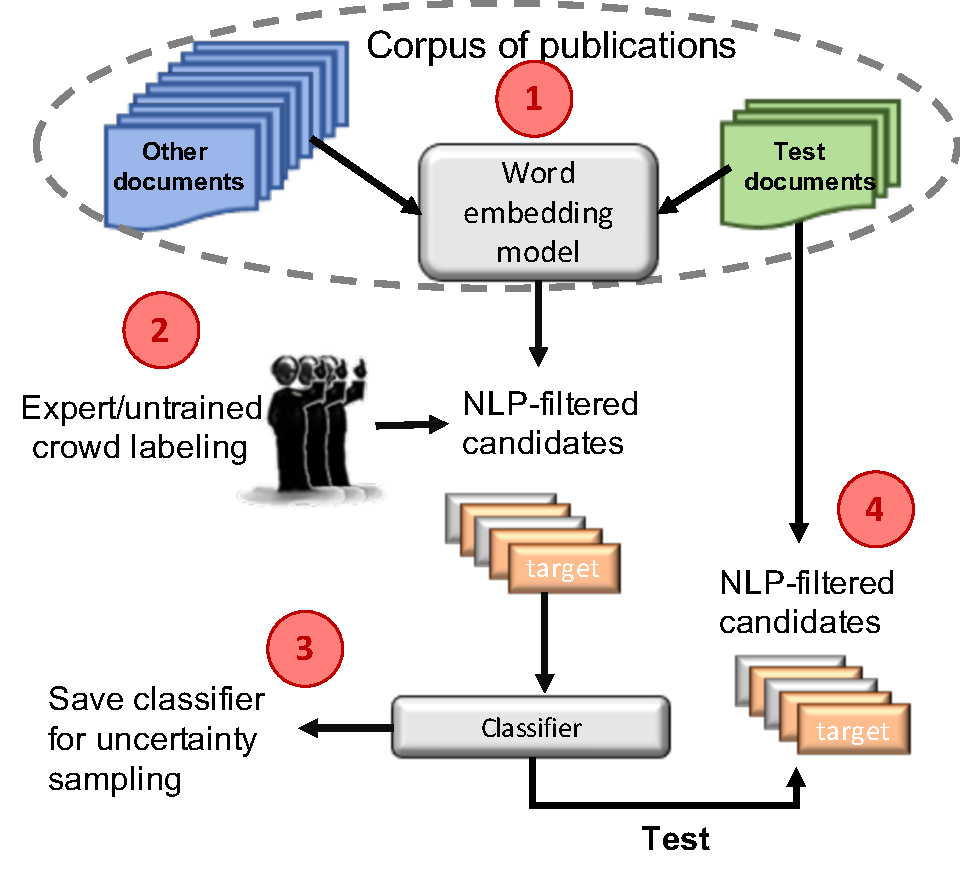
\includegraphics{figures/al_setup.pdf}}
\caption{\label{fig:current} The active learning experiment set up; we generate an unsupervised word embedding model using training documents in 1), we propose NLP-filtered candidate entities to untrained and expert annotators in 2) before classifying their word vectors in 3). The word embedding model is updated to include test documents in 4) and we verify results from step 3 using updated word vectors. Finally, we test this word vector classifier on all NLP-filtered words from the test documents in 6).}
%\kyle{more detail needed here. I think the pic is missing some arrows too. We could make it horizontal to ensure that it uses less space}\roselyne{I think addressed}.
%{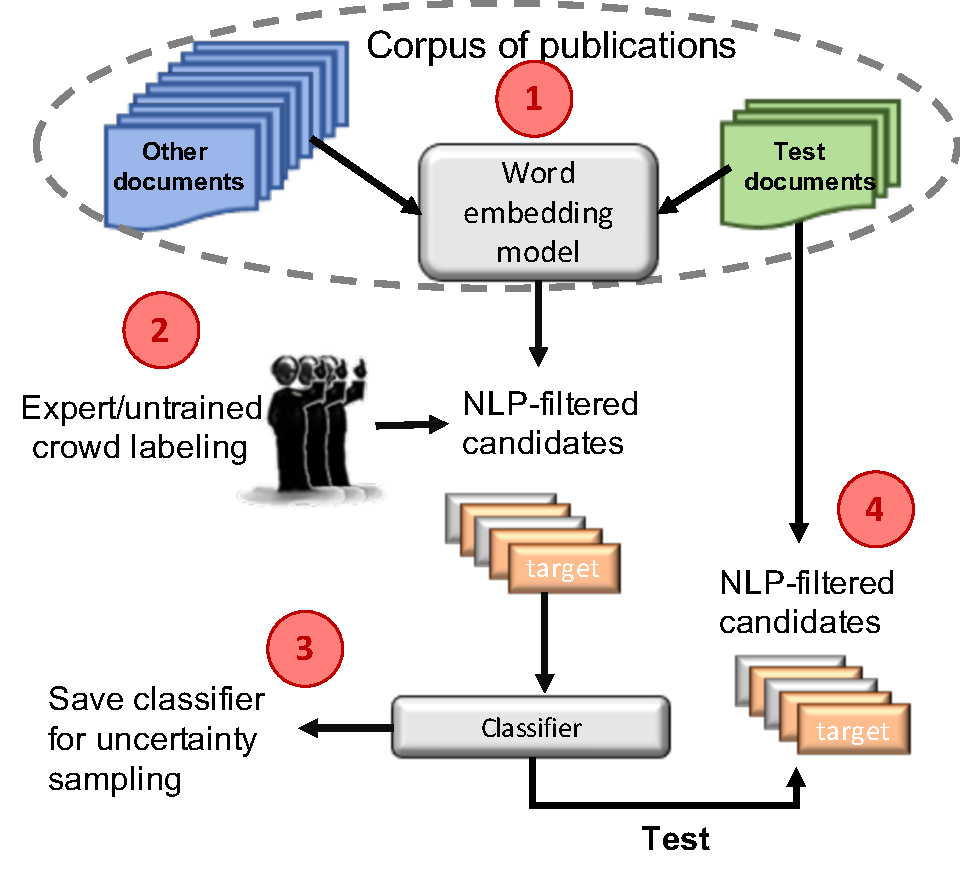
\includegraphics[trim=0in 4.in 0.1in 0,clip,width=\textwidth]{figures/al_setup.pdf}}
%\caption{\label{fig:current} The active learning process.
%}
\end{figure*}
`
\subsection{Active Learning Loop}
%\kyle{Confusing to have AL exp setup here}\roselyne{What if I change the name, I think I do have to put it here before the evaluation?}

Without prior knowledge of the distribution of target entities in the vector space, we use multiple of classifiers at each iteration of the active learning process. 
We save the best performing classifier on the labeled candidates for subsequent maximum entropy-based uncertainty sampling. 
The requested labels are annotated by humans to serve as addition training data for the next learning iteration. 
We describes these steps in more details in the following sections.\\

\subsubsection{Word Embedding Model}
We hypothesize that we can implement a classifier, which can detect word vectors for polymers based on their context. 
This, in turn, implies that word representation for polymers should not change considerably with small changes in corpora.
To test this hypothesis and separate our training and testing sets, we train our classifiers on vector representations of candidates generated from a word embedding model of a large set of training documents (see step 1 of Figure~\ref{fig:current}); 
we then update the classifier with our \textemdash smaller\textemdash test corpus and retrain the classifier. 
This validation step insures that there are no major differences in performance before and after the update (step 2 of Figure~\ref{fig:current}).
Finally, in step 3, we test our classifiers against all the NLP-filtered words from the test corpus, as shown on Figure~\ref{fig:current}.\\

\subsubsection{Untrained and Expert Labeling}
As explained in section~\ref{sect:background}, recognizing polymers can require more or less domain expertise.
We assign two domain experts to annotated candidates generated using our two maximum entropy-based uncertainty sampling (\textit{AL1} and \textit{AL2}). 
Each expert annotates one strategy but we perform crosschecking for 10\% of the first batch of labels. We confirm agreement between labels for all but 1 of the set of 20 candidates or an agreement of 95\%.
Experts simply approve or reject candidates using a simple web interface shown on Figure~\ref{fig:polyner}; a task that is more efficient than reading and annotating words in text.
The interface
provides example sentences as context for ambiguous candidates,
and allows the expert to access the publication(s) in which a particular candidate
appears when desired.

Expert time is costly and we aim to reduce the cost of obtaining labels.
Therefore for our baseline of randomly sampled NLP-filtered nouns, we experiment with a two-phase review process.
Tokenization can be a challenge for scientific entities such as polymers which contains characters such as `:', '\textendash', `,' etc. It can also generate other incoherent tokens from text, equations, captions etc.
For example, an untrained annotators may recognize that `$d\Sigma/d\Omega)(Q$' is not a polymer name and save time for the experts.
Hence, we assign two graduate student labelers to curate the candidates generated by the random sampling strategy, which is less likely to contain target entities.
First, the untrained labelers rejects obvious non-candidates via the previously mentioned web interface. 
Next, one of our expert polymer scientists indicates, for each remaining
candidate, whether or not it is in fact a polymer referent and submits a final review.
While we first used this two-phase review process for the random strategy, we envision generalizing and leveraging humans with different expertise through multi-phase reviews for all strategies to further save future costs.\\
%\kyle{Here we might want to think about positioning this as 2-phase review where we combine humans with different expertise levels}\roselyne{That's what I try to write about, I will specify that we did this for the random strategy but it could be applied to all strategies}


\begin{figure}
\centering
\frame{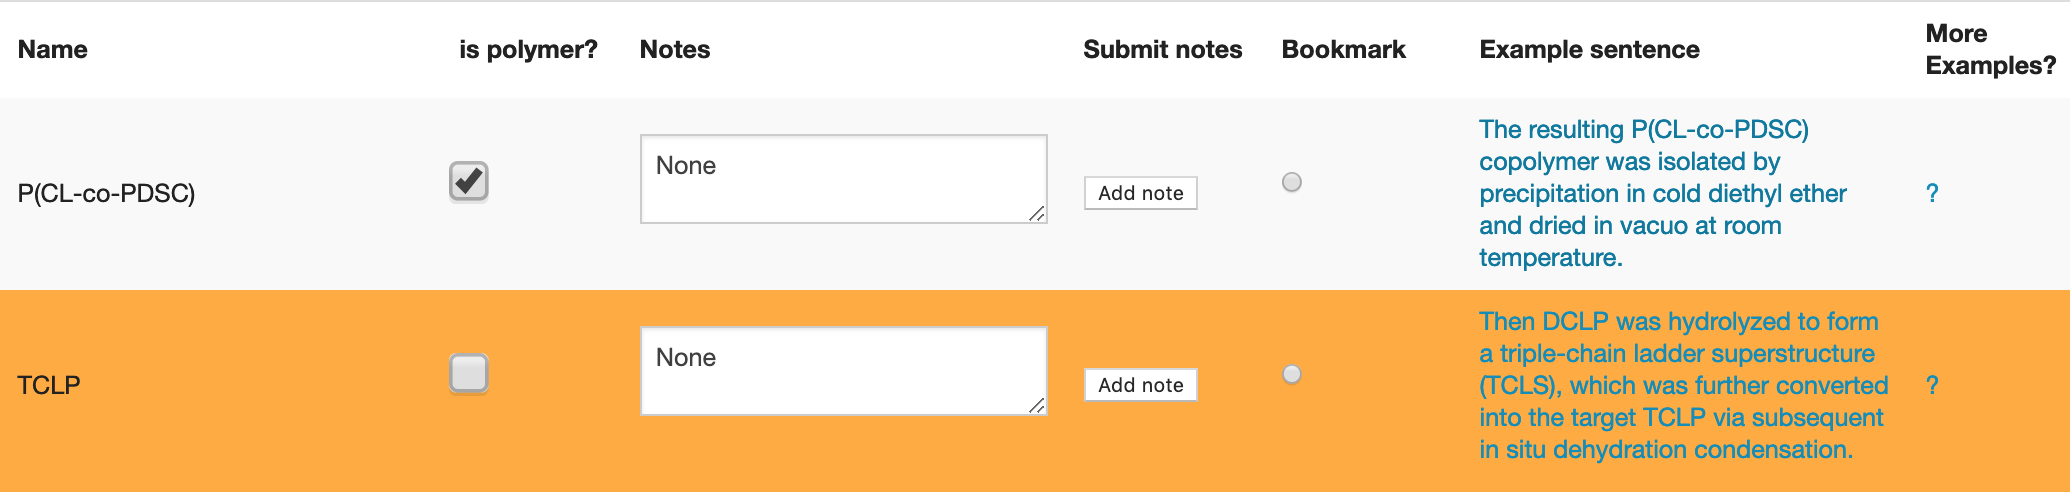
\includegraphics[trim=0in 0.1in 0.1in 0.in,clip,width=3.5in]{figures/expert_labeling.png}}
\caption{\label{fig:polyner} Web interface showing annotated candidates.
Clicking on ``?'' delivers up to 25 more example sentences.
}
\end{figure}

\subsubsection{Classification or Candidate Discrimination}
We use multiple of classifiers that we concurrently trained and test on the same data in steps 1, 2 and 3 illustrated on Figure~\ref{fig:current}.
The classifiers include the scikit-Learn implementations of Decision Tree (DT), Gradient Boosting (GB), K-Nearest Neighbor (KNN(uniform and distance weights)), Logistic Regression (LR), Linear Support Vector Machine (SVM), Naive Bayes (NB), and Random Forest (RF)~\cite{scikit-learn}. 
Our goal here is to explore the word embedding space and determine which classifier(s) works best for detecting our scientitic named entities.
As previously mentioned, we save the \textit{best-performing} classifier on labeled candidates (prior to updating the word embedding model  with test documents in order to clearly separate the training process from the test set, see step 1 in Figure~\ref{fig:current}).
When defining best performance, we prioritize retrieving a maximum of targets over precise extraction.
In other words, extracting a higher number of targets potentially requiring additional curation is favored over fewer correct targets.
In each case, we use the dimensions of the word vector for each string as input features.




